%%%%%%%%%%%%%%%%%%%%%%%%%%%%%%%%%%%%%%%%%%%%%%%%%%%%%%%%%%%%%%%%%%%
%
% This is a general template file for the LaTeX package SVJour3
% for Springer journals.          Springer Heidelberg 2010/09/16
%
% Copy it to a new file with a new name and use it as the basis
% for your article. Delete % signs as needed.
%
% This template includes a few options for different layouts and
% content for various journals. Please consult a previous issue of
% your journal as needed.
%
%%%%%%%%%%%%%%%%%%%%%%%%%%%%%%%%%%%%%%%%%%%%%%%%%%%%%%%%%%%%%%%%%%%
%
\RequirePackage{fix-cm}
%
\documentclass[twocolumn]{svjour3}
%
\smartqed
%
\usepackage{graphicx}
\usepackage[T1]{fontenc}
\usepackage{hyperref}
\usepackage[round, sort&compress, numbers]{natbib}
\usepackage{multirow}
\usepackage{graphicx}
\usepackage{units}
\usepackage{color}
\usepackage{xspace}
%
\DeclareRobustCommand\IPCClongname{}
%
% please place your own definitions here and don't use \def but \newcommand{}{}
\newcommand{\pmlib}{\texttt{pmlib}\xspace}
%
% Insert the name of "your journal" with
% \journalname{myjournal}
%
\begin{document}

\title{Evaluating the Performance and Energy Efficiency of COSMO-ART,
  a Coupled Numerical Weather Forecast and Chemical Transport Model.}
%\thanks{}
%\subtitle{}

%\titlerunning{Short form of title} % if too long for running head

\author{Joseph~Charles \and William~Sawyer \and Manuel~F.~Dolz \and
  Sandra~Catal\'an}

%\authorrunning{Short form of author list} % if too long for running
%head

\institute{J.~Charles, W.~Sawyer
	\at Swiss National Supercomputing Centre (CSCS)
	\\ CH-6900 Lugano, Switzerland
 	\\ E-mails:~{\{joseph.charles,william.sawyer\}@cscs.ch}
        \and M.~F.~Dolz
        \at Dept. of Informatics, University of Hamburg (UHAM)
	\\ DE-22527 Hamburg, Germany
        \\ \email{manuel.dolz@informatik.uni-hamburg.de}
        \and S.~Catal\'an
        \at Jaume I University of Castell\'on (UJI)
	\\ ES-12071 Castell\'on, Spain
        \\ \email{catalans@icc.uji.es}
}

\date{Received: date / Accepted: date} % The correct dates will be
                                       % entered by the editor

\maketitle

\begin{abstract}
  In  this paper we  present the  energy-to-solution and  profiling of
  COSMO-ART on various  platforms.  This model is an  extension of the
  operational  weather forecast  model of  the German  weather service
  (DWD), developed for the  evaluation of the interactions of reactive
  gases  and aerosol  particles with  the state  of atmosphere  at the
  regional scale.  The overall  performance of this application on HPC
  systems is analysed  by a profiling study to  determine hotspots and
  identify  critical  CPU paths.   Moreover,  we describe  measurement
  devices and energy-aware techniques  employed to evaluate the energy
  footprint of the considered application and to get detailed insights
  about power bottlenecks.  Our motivation is to improve corresponding
  code    sections   to    sustain   performance    while   minimising
  energy-to-solution.   This  preliminary  work  sets  the  basis  for
  subsequent studies to tackle  challenges related to energy efficient
  high performance computing in the framework of the Exa2Green project
  (\url{http://exa2green.eu/}).

\keywords{High performance computing  \and Energy-aware computing \and
  Green computing  \and Numerical weather  prediction \and Atmospheric
  chemistry  \and  Aerosols  modelling  \and  Profiling  methods  \and
  Benchmark    analysis   \and    COSMO-ART    coupled   model    \and
  Time-to-solution \and Energy-to-solution \and Xeon processor}
% \PACS{PACS code1 \and PACS code2 \and more}
% \subclass{MSC code1 \and MSC code2 \and more}
\end{abstract}

\section{Introduction}
\label{intro}
The  interaction  between aerosols  and  clouds  presents  one of  the
biggest  uncertainties  in   present  day  climate  simulations.   The
chemistry involved is complex,  but there is a concerted international
effort to model the underlying processes through models. These models,
such as  the Aerosol  Reactive Transport (ART),  developed at  the KIT
(Karlsruhe  Institute of  Technology)  , offer  a  key opportunity  to
reduce   the  climate  uncertainty,   particularly  on   the  regional
scale. These  models can be coupled  with climate models,  such as the
regional  weather  and   climate  COSMO  (Consortium  for  Small-scale
Modelling) model  developed by the German Weather  Service (DWD).  The
COSMO model  is a weather forecast  model which has  become a standard
all  over Europe.   Beside the  federal weather  forecast  stations in
Germany  (Deutscher  Wetterdienst,  DWD),  Switzerland  (MeteoSchweiz,
MCH),  Italy (Ufficio  Generale  Spazio Aereo  e Meteorologia,  USAM),
Greece  (Hellenic   National  Meteorological  Service,   HNMS)  Poland
(Institute  of   Meteorology  and  Water   Management,  IMGW)  Romania
(National  Meteorological  Administration,  NMA) and  Russia  (Federal
Service for Hydrometeorology  and Environmental Monitoring, RHM), also
a   large  number   of  agencies   including  military   and  research
institutions  base their  forecasts on  COSMO. The  combined COSMO-ART
model is capable of simulating  aerosol distributions as well as their
interactions over Europe as well as other regional domains.

It has  been a major  scientific achievement to effectively  model the
underlying  chemical  processes   through  these  applications.   This
achievement  now   needs  to  be  fostered  by   reducing  its  energy
expense. Currently, resource allocation  is one of the key limitations
to scientists  in running the simulation periods  and resolutions they
would like.


\section{Related work}
\label{sec:1}
While the  TOP500 list was  introduced over 20  years ago to  rank the
performance of HPC systems worldwide, it is quite recently that energy
efficiency  become  a  critical  constraint  in the  way  to  exascale
computing.   Since 2007,  the Green500  power  measurement methodology
encourages the design,  procurement and management of energy-efficient
infrastructures   to  contain   performance  in   an   affordable  and
competitive  power envelope.   However, the  state-of-the-art research
assessing performance  and energy efficiency of  applications is still
scarce.

\emph{Padoin et al.}   \cite{Padoin-2013} investigate performance and
power  consumption  of  an  agroforestry  application  and  show  that
changing workload  can drastically improve energy efficiency  of CPU +
GPU heterogeneous architectures.

\emph{Ou  Pang et  al.}   \cite{Ou-2012} compare  ARM  and Intel  x86
workstations  clusters  and   conclude  that  ARM-based  clusters  are
advantageous  with   lightweight  applications  in   terms  of  energy
efficiency.

\emph{G\"oddeke et al.}  \cite{Goddeke-2013} evaluate weak and strong
scalability of PDE solvers on a cluster of 96 ARM dual-core processors
and demonstrate  that the ARM-based  cluster can be more  efficient in
terms of energy-to-solution compared to x86-based cluster.

\emph{Wittmann  et  al.}   \cite{Wittmann-2013}  perform  a  thorough
analysis of  a lattice-Boltzmann method based CFD  simulation on Intel
Sandy   Bridge  processors   and  show   extrapolated  results   on  a
petascale-class machine.

\emph{Cumming  et  al.}  \cite{Cumming-2014}  present  a simple  and
practical  methodology  looking at  energy  minimization  that can  be
applied to various applications.


\section{The COSMO-ART model system}
\label{sec:2}
\subsection{Model Description}
\label{subsec:1.1}
The  model  system COSMO-ART  described  in  \citep{Vogel-2009}, is  a
regional  to  continental scale  model  coupled  online  to the  COSMO
numerical weather  prediction and climate  model \citep{Baldauf-2011}.
It  incorporates  sophisticated  modules  for  gaseous  chemistry  and
aerosol dynamics  and allows the online calculation  of reactive trace
substances    and    their    interaction    with    the    atmosphere
\citep{Knote-2011}.  Detailed  model   description  can  be  found  in
\citep{Stanelle-2010, Bangert-2012, Knote-2011, Knote-2013}.

\subsection{Model Setup}
\label{subsec:1.2}
Establishing effective energy performance benchmarking of a code under
intense development such as COSMO-ART is a challenging task because of
the  absolute necessity that  results must  be reproducible  within an
expected  variance for the  duration of  the Exa2Green  project. After
consultation  with  the  climate  community  to  properly  define  the
baseline,  it was  necessary to  find a  run-configuration  capable of
being recreated in all subsequent versions of the code.

Thus, we give here a brief  overview of the main features of the model
setup for  our benchmark's daily  runs.  Three-dimensional simulations
are performed over  Europe for April 13th 2010, which  is close to the
equinox and thus  brings benefits of having approximately  half day of
night  and half  day  of  sun exposure,  therefore  ensuring a  proper
activation of the chemistry cycle. We consider daily 24-hour forecasts
without  any  previous spin-up  simulations.   The calculation  domain
corresponds to  the CORDEX-EU-44  domain and is  covered by a  grid of
$222\times   216$    points   with   a    horizontal   resolution   of
$0.22\,^{\circ}$,  i.e.  50  km in  both directions,  and  40 vertical
layers.  COSMO-ART requires the following input data:

\begin{itemize}
\item  Gas phase:  Anthropogenic emissions  for different  species and
  land use data for biogenic emissions and deposition,
\item Aerosol particles: Anthropogenic emissions,
\item Mineral dust: Soil specific land use data.
\end{itemize}

The meteorological initial and  bounday conditions are obtained by the
the ECMWF  global spectral model IFS  with an update  frequency of 3h.
Boundary data  for gas-phase species are taken  from IFS-MOZART output
at   6h  temporal   resolution.   NAMELIST-input   specifying  runtime
parameters    splitted   into    several   groups    are    given   in
Table~\ref{tab:1}.   The model setup  incorporates 34  2-d and  45 3-d
fields  to  be  written  out  every  hour  and  doesn't  include  data
assimilation methods.

\begin{table}[htbf]
  \begin{center}
    \caption{}
    \label{tab:1}
    \begin{tabular}{ll}
      \hline\noalign{\smallskip} 
      \textbf{Group} & \textbf{Description} \\
      \noalign{\smallskip}\hline\noalign{\smallskip}
      LMGRID & Grid domain and size parameters \\
      RUNCTL & Model run parameters \\
      TUNING & Physics and dynamics parameters \\
      DYNCTL & Adiabatic model parameters \\
      PHYCTL & Diabatic model parameters \\
      COSMO\_ART & Gases and aerosols model parameters \\
      DIACTL & Diagnostic calculations parameters \\
      SATCTL & Synthetic satellite images parameters \\
      IOCTL & I/O environment parameters \\
      GRIBIN & GRIB input parameters \\
      GRIBOUT & GRIB output parameters \\
     \noalign{\smallskip}\hline
    \end{tabular}
  \end{center}
\end{table}

This COSMO-ART version is configured with a semi Lagrangian horizontal
advection  scheme with  tricubic interpolation  and  selective filling
diffusion  option  in  combination   with  the  dynamical  core  using
Runge-Kutta time stepping \citep{}.  It  also makes use of the Kinetic
PreProcessor solver (KPP) for  the resolution of atmospheric chemistry
ordinary  differential equations \citep{Damian-2002}.   Concerning the
modelling  of  wet  deposition  in  aerosols, the  baseline  has  only
indirect  cloud  feedbacks  but  doesn't include  in-cloud  scavenging
(rainout) and below-cloud  scavenging (washout) yet.  Amongst physical
parameterisations,   precipitation  formation   is   performed  by   a
two-moment  cloud  microphysics scheme  instead  of  a classical  bulk
microphysics scheme.


\section{Power-performance measurement framework}
\label{sec:3}
In this section,  we present two different frameworks  deployed on HPC
systems  to  measure the  power  consumption  and  performance of  the
baseline execution.

\subsection{Framework description}
\label{subsec:3.1}

\subsubsection{CSCS - E3METER metering products}
Supercomputer  clusters considered  for our  experiments at  the Swiss
National Supercomputing Center of  ETH Zurich (CSCS) are equipped with
E3METER Intelligent  Power Strips (IPS)  and Monitors (IPM)  which are
high   quality   electricity  meters   released   by  Riedo   Networks
(\url{http://riedonetworks.com/}),  that  enable  to monitor  and  log
power  consumption of  the  IT infrastructure  as  well as  constantly
analyze  line  voltage,  current,  power-factor,  frequency  with  1\%
accuracy.   Using reliable  narrowband  powerline communication  (PLC)
technology,  all metering  and power  quality data  from each  IPS are
centrally collected by the E3METER Data Concentrator, via the existing
power cables thus  avoiding the need for extra  cabling.  This data is
made  available  via SNMP,  HTTP,  TELNET  through  the built-in  Fast
Ethernet  port.   Time  synchronisation  is guaranteed  by  using  NTP
servers.   Measured data  is accessed  through the  open  source Cacti
software including  the E3METER  Cacti Plugin to  scan the  entire PLC
network and monitor  in real-time the power usage  of individual rack,
recorded in 5 minutes interval periods.

\subsubsection{University of Hamburg}
To assess the  performance and the energy efficiency  of COSMO-ART, we
employ   a    version   of   the    integrated   framework   presented
in~\cite{energy13} that works in  combination with Extrae and Paraver,
which are profiling/tracing and visualization tools, respectively.

%The left part of the \vref{fig:Lustre} offers a graphical representation of
%the Lustre architecture; the right depicts the tracing and profiling framework.
To use our  approach, COSMO-ART is compiled using  the Extrae compiler
wrappers,  which  automatically instrument  the  Fortran  code of  the
model. Next, COSMO-ART  is run on the nodes,  thus dissipating certain
amount  of power.   These  nodes are  connected  to power  measurement
devices that account for the dissipated power/consumed energy and send
the power  data to the  tracing server.  The client,  meanwhile, sends
start/stop  primitives  in  order  to  gather  captured  data  by  the
watt-meters onto the  tracing server, where an instance  of the \pmlib
server is running.

Once COSMO-ART run is finished, a file containing the power profile is
created using the power data  received from the tracing server and the
instrumentation post-processing generates the performance trace files.
All  these files  are  combined then  in  Paraver which  allows us  to
visualise the performance trace and the power profile of COSMO-ART all
together.

%Once COSMO-ART run is finished, the VampirTrace \pmlib plugin receives
%the  power   data  from  the  tracing   server.   The  instrumentation
%post-processing generates  the performance trace files  and the \pmlib
%plugin inserts the power data into them.

%In  addition  to the  power  measurements,  we  also account  for  the
%resource utilization values  of the nodes: CPU load,  memory usage and
%storage device utilization. % and network utilization.

%We  run special  \pmlib  server  instances on  the  server nodes  that
%retrieve these  values from the \texttt{proc}  file system (leveraging
%the  \texttt{psutil} Python library).   Thus, \pmlib  plugin instances
%running  with the  instrumented  application connect  with the  \pmlib
%servers.   Finally,   using  the   Vampir   visualization  tool,   the
%power-performance traces  can be easily  analyzed through a  series of
%plots and statistics.


\section{Evaluation}
\label{sec:4}
In  this  section, we  present  a  performance  and energy  efficiency
evaluation  of  different  achitectures  when  running  the  COSMO-ART
baseline.  We  start by  specifying our measurement  methodology along
with the metrics used to  analyse the results on all platforms.  Then,
we detail the environment  setup gathering the considered HPC systems,
the software  environment and the runtime  configuration.  Finally, we
discuss  benchmark   results  and  power-performance   traces  of  the
application.

\subsection{Measurement methodology}
\label{subsec:4.1}
To analyse the energy  footprint and overall performance of COSMO-ART,
two  important metrics  were  examined: \textit{time-to-solution}  and
\textit{energy-to-solution}.   Time-to-Solution  refers  to the  total
wall clock time of  the application execution time. Energy-to-solution
is the amount  of energy spent to achieve  results. Energy consumption
of CSCS clusters is assessed  by sampling the instantaneous peak power
during  execution  which  is  then  averaged  and  multiplied  by  the
time-to-solution  to determine energy-to-solution.  Whenever possible,
multiple production runs of COSMO-ART were performed to illustrate the
reproducibility  of   the  baseline,  and   quantify  the  significant
uncertainties in  the power measurement, as dictated  by the available
technology.

\subsection{Environment setup}
\label{subsec:4.2}
While hardware  platforms mature  and are replaced,  we have  chosen a
state-of-the-art  Intel's  third-generation   Core  (aka  Ivy  Bridge)
processing platform (called ``Monch'')  for our power measurements, as
it  is slated  to stay  in service  without hardware  upgrade  for the
duration  of  the Exa2Green  project.   In  principle  at least,  this
architecture could be recreated or found in an identical configuration
beyond the lifetime of the project.  Given that the baseline benchmark
can be reproduced  within an expected variance, and  that the baseline
run configuration  can be used in  all future versions of  the code, a
fair comparison  will be made  between the baseline and  the milestone
versions   of    COSMO-ART.    In   this    study,   a   complementary
energy-to-solution  benchmarking  comparison  is  carried out  on  the
``Pilatus'' cluster based  on Intel's previous-generation Sandy Bridge
processors, conventional  in HPC  systems and known  to be  more power
consuming.

\subsubsection{Monch (CSCS - ETH Zurich)}
Monch, which is installed  at the Swiss National Supercomputing Center
(CSCS) of ETH Zurich, is  a 10 rack NEC-provided and dual-socket Intel
Ivy Bridge-EP based cluster, utilised from people that are part of the
Swiss    Platform   for    Advanced   Scientific    Computing   (PASC,
\url{http://www.pasc-ch.org/}). It is composed of 312 standard compute
nodes, 24 large-memory compute nodes and 24 huge-memory compute nodes.
Each standard  compute node comprises two Intel  Ivy Bridge-EP E5-2660
v2 ten-core processors operating at 2.2 GHz, themselves connected by a
high speed  InfiniBand network, based  on Mellanox SX6036  managed FDR
switches, with a  56 Gb/s speed.  Each core has  32 KB instruction and
32 KB data L1  caches and 256 KB of L2 cache. All  the 10 core share a
25 MB L3 cache and the platform has 32GB of DDR3 1600 MHz RAM. For our
energy-to-solution benchmark,  a full rack of Monch  constituted of 52
standard  compute   nodes  (monchc[029-080])  was   considered.

\subsubsection{Pilatus (CSCS - ETH Zurich)}
Pilatus,  which  is installed  at  the  Swiss National  Supercomputing
Center (CSCS)  of ETH Zurich,  is a dual-socket Intel  Sandy Bridge-EP
based cluster  used as Piz  Daint pre-post processing cluster.   It is
composed of 42 compute nodes  and has 2 high-speed interconnects based
on FDR:  the first is dedicated to  the MPI traffic and  the second to
the storage high speed traffic.  The 2 login nodes and the 42 computes
nodes  consists in  11  twin-pair Intel  E5-Series  DALCO r2264i4t  2U
scalable compute modules.  Each  module contains 4 compute nodes based
on two Intel Xeon E5-2670  eight-core processors operating at 2.6 GHz,
themselves  connected by  a high  speed InfiniBand  network,  based on
Mellanox SX6036 managed FDR switches,  with a 56 Gb/s speed. Each core
has 32 KB instruction and 32 KB data L1 caches and 256 KB of L2 cache.
All the  8 core share a  20 MB L3 cache  and the platform  has 64GB of
DDR3 1600 MHz  RAM. For our energy-to-solution benchmark,  a full rack
of Pilatus  constituted of 42 standard  compute nodes (pilatus[03-44])
was considered.

\subsubsection{Sofware environment}
INT2LM  and the  COSMO-ART model  are  implemented in  Fortran 90  for
distributed  memory  parallel  computers  using  the  Message  Passing
Interface (MPI)  and are purely  MPI-parallel.  The software  stack on
both many-core  platforms was  controlled using the  modules framework
which gives  an easy and  flexible mechanism to  access to all  of the
CSCS  provided compilers,  tools  and applications.   For our  initial
benchmarking,  we opted  for  the GNU  compiler  (gcc/4.8.1 on  Monch,
gcc/4.8.2 on Pilatus) with the -O3 compiler flag as it generally gives
a  good  level  of optimization  and  the  code  runs faster  in  this
configuration  than when  compiled with  the intel  compiler (14.0.1).
Besides, we installed the  MPICH2 implementation of MPI (mvapich2/1.9)
as  well  as  the  commonly  used HDF5  (1.8.12)  and  NetCDF  (4.3.1)
libraries in favor of the  traditional GRIB library for the management
of extremely  large and complex data collections.   All computes nodes
have    an   operating   system    based   on    GNU/Linux   featuring
``2.6.32-358.11.1.el6.x86\_64''  and  ``3.0.101-0.15-default'' kernels
for Monch and Pilatus respectively.

\subsubsection{Run configuration}
A snapshot of the code, which includes, at least conceptually, all the
information needed  to reproduce the  energy-to-solution benchmarks of
COSMO-ART, was produced and run on a 1040 cores using 20 MPI tasks per
node on  Monch and  on a  1344 cores using  16 MPI  tasks per  node on
Pilatus.   The  calculated  region  was mapped  to  the  participating
processors using  a 2D-partitioning strategy.   The distribution along
the  x and  y  coordinates  was defined  by  setting: $nprocx=40$  and
$nprocy=26$ for  Monch and $nprocx=28$ and $nprocy=24$  as $nprocx$ is
usually  kept  bigger  than  $nprocy$.   Besides as  this  version  of
COSMO-ART  doesn't  make  use   of  the  GRIB  library,  we  specified
$nprocio=0$ for  GRIB I/O.  Hyperthreading  is not considered  in this
study as previous  attempts of its use revealed that  it always led to
higher energy-to-solution.\\

\subsection{Experimental results}
\label{subsec:4.3}

\begin{figure}[htbf]
  \begin{center}
    \includegraphics[width=0.48\textwidth]{Figs/NRJ_benchmark_Monch.eps}
    \caption{Monch: Isola E1 Rack 2 Total Power}
    \label{fig:1}
  \end{center}
\end{figure}

\begin{figure}[htbf]
  \begin{center}
    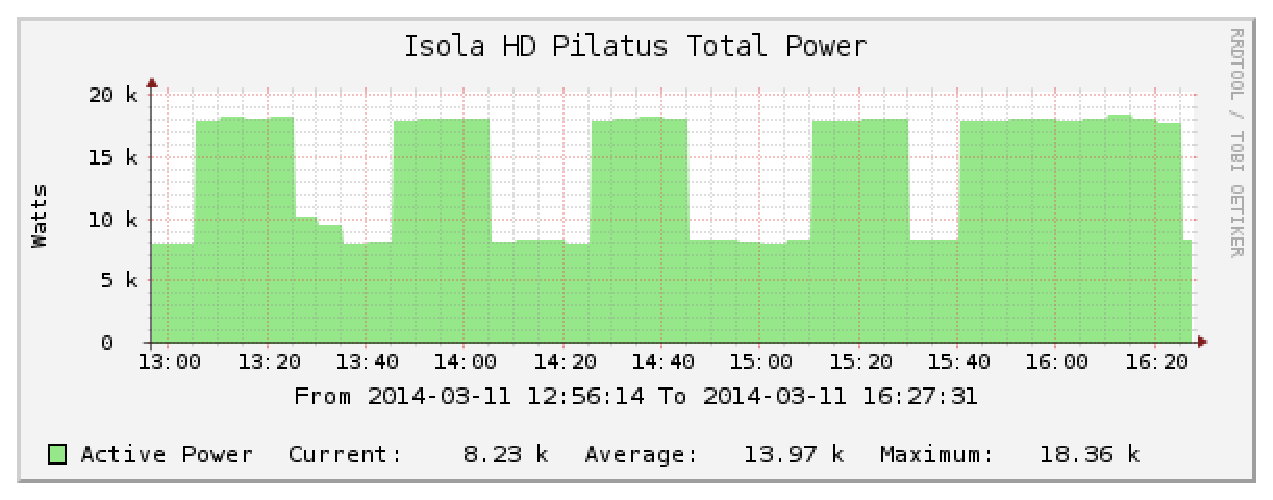
\includegraphics[width=0.48\textwidth]{Figs/NRJ_benchmark_Pilatus.eps}
    \caption{Pilatus: Isola HD Total Power}
    \label{fig:2}
  \end{center}
\end{figure}

Figures~\ref{fig:1} and  \ref{fig:2} account respectively  for Monch's
Isola E1  Rack 2  and Pilatus' Isola  HD total power  measurements for
1-day or 2-days simulations. On  the Intel Ivy Bridge EP based cluster
(i.e. Monch), the 1-day simulation  was issued only twice due to usage
restrictions. As time resolution was set to one update every 5 minutes
for  power sampling,  the average  power consumption  was  computed by
considering 6 values for each single  run.  On the Intel Xeon E5 based
cluster (i.e.   Pilatus), the 1-day  simulation was issued  four times
and a 2-days  run only once. Similarly, the  average power consumption
was computed by  considering 4 values for each single  1-day run and 9
values  for the  2-days  run. Corresponding  results  are gathered  in
Table~\ref{tab:3}.

\begin{table}[htbf]
  \begin{center}
    \caption{Average power consumption (W) of the platforms}
    \label{tab:3}
    \begin{tabular}{ccc}
      \hline\noalign{\smallskip}
      \textbf{Simulation time} & \textbf{Xeon E5} & \textbf{Ivy Bridge EP} \\
      \noalign{\smallskip}\hline\noalign{\smallskip}
      \textbf{1 day} & 18122.01417 & 12658.52278 \\ 
      & 17979.61083 & 12586.40833 \\
      & 18065.45167 & - \\
      & 17973.02833 & - \\
      \noalign{\smallskip}\hline\noalign{\smallskip}
      \textbf{2 days} & 17997.57815 & - \\
      \noalign{\smallskip}\hline
    \end{tabular}
  \end{center}
\end{table}

In Figure~\ref{fig:3}, we compare both time-to-solution (right y-axis)
and  energy-to-solution (left  y-axis) metrics  on both  platforms. As
expected,  Xeon  E5 outperforms  Ivy  Bridge  EP,  being roughly  1.3x
faster.  The reason for that is twofold: it has higher clock frequency
than Xeon E5 (2.6 GHz against  2.2 GHz) and it aims at computing speed
regardless to  energy consumption. In  our experiments, Ivy  Bridge EP
showed the best energy-to-solution, reducing the energy consumption of
Xeon E5 by approximately $7\%$.

\begin{figure}[htbf]
  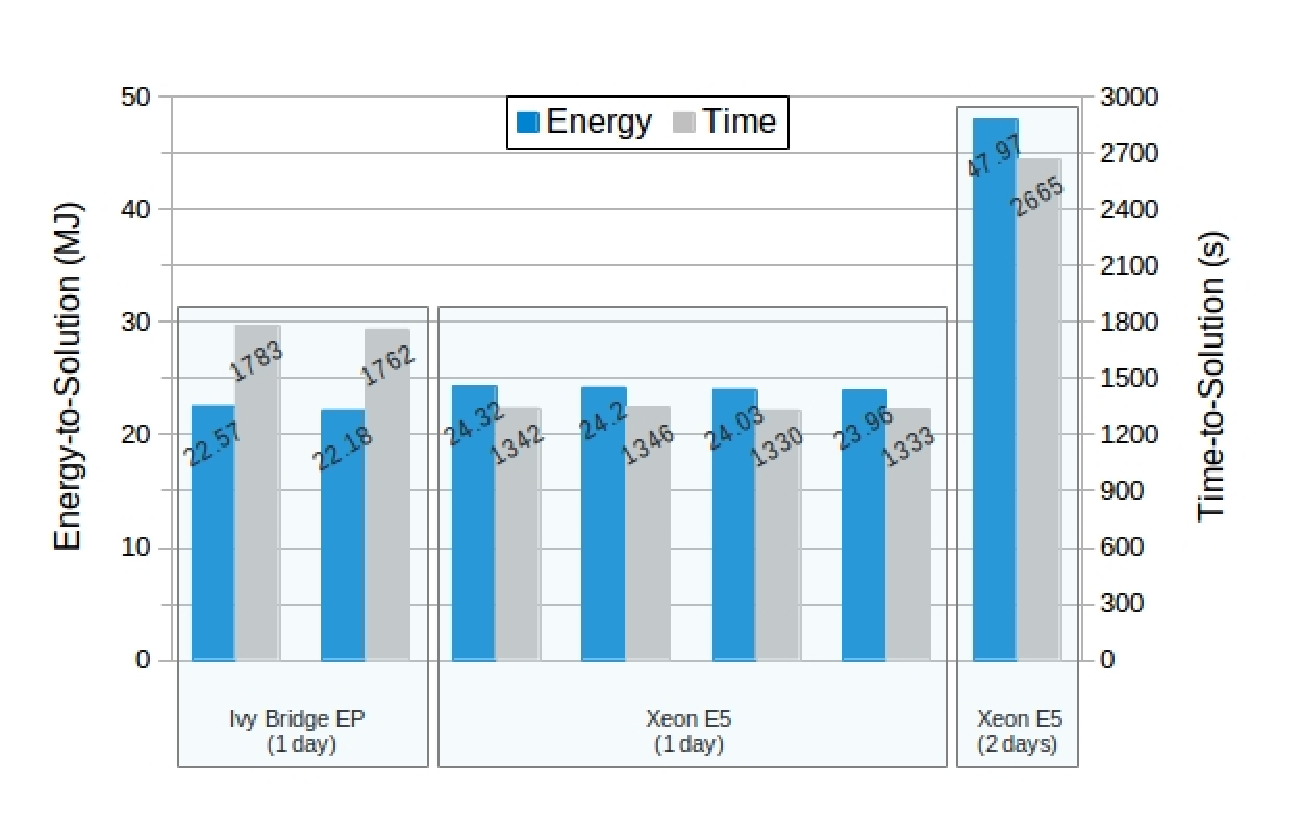
\includegraphics[width=0.5\textwidth]{Figs/Time_E2S_COSMO-ART.eps}
  \caption{Time-to-solution and  energy-to-solution comparison between
    Xeon E5 and Ivy Bridge-EP architectures}
  \label{fig:3}
\end{figure}




















\section{Conclusion}
\label{concl}
We  have   presented  a  methodology  for   comparing  performance  of
COSMO-ART,  a  regional  weather  forecast  model  augmented  for  the
interactions of  reactive gases and aerosol  particles.  The resulting
benchmarks illustrate  that the  best time-to-solution does  not imply
the best energy-to-solution: an Intel Sandybridge (2.6 GHz) system has
lower  time-to-solution but  higher energy-to-solution  than  an Intel
Ivybridge  (2.2  GHz) system,  although  the  two  metrics are  indeed
strongly  correlated.   A   tool  utilising  Paraver/Extrae  with  new
extensions  for power  consumption  was successfully  applied to  this
non-trivial application.  The  resulting profiles indicate that simple
changes, such as making use of an MPI version based on blocking rather
than polling, can reduce power consumption significantly.

This  reproducible  benchmark provides  a  baseline  for ongoing  work
package within  the EU-funded Exa2Green to  minimise power consumption
of COSMO-ART. Profiling  has given us insight into  the most expensive
code  components,  which are  now  being  altered  to utilise  revised
algorithms.  The  results of these  optimisations will be  reported in
future publications.


%\paragraph{Paragraph headings} Use paragraph headings as needed.

\begin{acknowledgements}
The research  leading to these  results is supported by  the Exa2Green
project  co-financed by  the European  Commission under  7th Framework
Programme Future and Emerging Technologies (FET) Proactive Initiative:
Minimising Energy  Consumption of Computing to the  Limit (MINECC). We
also gratefully acknowledge the High Performance and High Productivity
Computing  Initiative  (\url{www.hp2c.ch}) for  results  that will  be
leveraged in subsequent code refactoring.
\end{acknowledgements}

\DeclareRobustCommand\IPCClongname{ - Intergovernmental Panel on Climate Change}

\bibliographystyle{plainnat}
\bibliography{\jobname}

\end{document}

